\documentclass[a4paper,12pt]{book}

% PACKAGES

\usepackage{afterpage}
\usepackage{amsmath}
\usepackage[utf8]{inputenc}
\usepackage{chngcntr}
\usepackage{blindtext}
\usepackage[labelsep=space]{caption}
\usepackage{enumitem}
\usepackage{fancyhdr}
\usepackage[T1]{fontenc}
\usepackage[bottom=6.5em]{geometry}
\usepackage{graphicx}
\usepackage{gensymb}
\usepackage[hyperfootnotes=false,linktoc=page,pdfpagelayout=TwoPageRight]{hyperref}
\usepackage{lettrine}
\usepackage{cfr-lm}
\usepackage{makecell}
\usepackage{mathtools}
\usepackage{multicol}
\usepackage[defaultlines=4,all]{nowidow}
\usepackage{titlesec}
\usepackage{tocloft}
\usepackage{wrapfig}
\usepackage{listings}
\usepackage{xcolor}
\usepackage[pages=some]{background}

\backgroundsetup{
scale=1,
color=black,
opacity=0.9,
angle=0,
contents={
  
\includegraphics[width=0.6\textwidth]{img/cover.png}
  }
}

\lstset
{ %Formatting for code in appendix
    language=Python,
    basicstyle=\footnotesize,
    numbers=left,
    stepnumber=1,
    showstringspaces=false,
    tabsize=1,
    breaklines=true,
    breakatwhitespace=false,
}

\usepackage{hyperref}
\hypersetup{
    colorlinks=true,
    linkcolor=blue,
    filecolor=magenta,      
    urlcolor=cyan,
    pdftitle={Overleaf Example},
    pdfpagemode=FullScreen,
    }

\counterwithin*{footnote}{page}

% FIGURES

\newcommand{\fig}[3]{
    \begin{figure}[h]
        \centering
        \includegraphics[width=\linewidth]{#1}
        \textbf{\caption{#2}}
        \label{fig:#3}
    \end{figure}
}

% REFERENCES

% TABLE OF CONTENTS FORMAT

\renewcommand{\contentsname}{CONTENTS}
\renewcommand{\cfttoctitlefont}{\hfil\bfseries\fontsize{15pt}{0pt}\selectfont}
\renewcommand{\cftaftertoctitleskip}{0.5\baselineskip}
\renewcommand{\cftsecfont}{\bfseries}

\addtolength{\cftsecnumwidth}{40pt}
\addtolength{\cftsubsecnumwidth}{10pt}
\setlength{\cftbeforetoctitleskip}{-3em}

\setcounter{tocdepth}{4}
\setcounter{secnumdepth}{4}

% TITLE SETUP

\title{\textbf{\huge{Static Program Analysis}\\ \vspace{1cm}\Large{Version 0.1a} \\ \vspace{10cm}\Large{Michael Canesche}}}

%\author{
%    Secondary Author
%    \and
%    Tertiary Author
%}

%\date{}

% DOCUMENT

\begin{document}

% TITLE
\BgThispage
\maketitle
\clearpage

% PREFACE
\newpage
\begin{center}
    \textbf{\Large{PREFACE}}
\end{center}

This book was based on Professor Fernando Magno Quintão's material. You can access the material at this \hyperlink{https://homepages.dcc.ufmg.br/~fernando/classes/dcc888/}{link} and other materials on the website (Please always look in the end of chapter for reference). Fernando was my advisor during my Ph.D., and He created and taught the course DCC888 – Static Program Analysis at UFMG, which I had the pleasure to do. Of course, this book doesn't have the goal to substitute the original material, but maybe complement it. I strongly recommend you read and study the material created by him.

But, Michael, why are you taking so long to finish the book? The image below answers your question :)

\begin{figure}[!ht]
    \centering
    
\includegraphics[width=0.5\textwidth]{img/dragon.png}
\end{figure}

Do you want to contribute with this material and receive a baby dragon medal and a special thank you by me? Please send me an e-mail (michael.canesche@gmail.com). We can chat and talk about compiler and other stuff! :D 

\vspace{\baselineskip}

\textit{\today} \hfill Michael Canesche

% TABLE OF CONTENTS

\pagenumbering{gobble}
\pagestyle{empty}
\newgeometry{bottom=6em}
    \renewcommand{\baselinestretch}{0.94}\normalsize
            \tableofcontents
    \renewcommand{\baselinestretch}{1.0}\normalsize
\restoregeometry
\pagestyle{fancy}

\clearpage

% CONTENTS

\pagenumbering{arabic}

\chapter{Introduction}
\label{ch:intro}

In this chapter, We will focus on the main subjects of static program analysis. 
Section \ref{sec:comp} we talk about us, the compiler guys. 
Section \ref{sec:analysis} is about the comparison between static and dynamic analysis. 
In the next section \ref{}, we want to show some applications in real life.  

\section{The Compiler Guys and Where We're Going}
\label{sec:comp}

Someone in one place and one time was thinking about how to save time for millions of programmers, and the answer was simple: Let's build a Compiler! The goal of a compiler writer is to bridge the gap between programming languages and the hardware; hence, making programmers more productive. This book is not about creating our own compiler. But, your knowledge of compiler will be welcome here. Well, let's start to present the main goals of this book.

\begin{itemize}
    \item Explain to the student how to transform a program automatically, while preserving its semantics, in such a way the new program is more efficient according to a well-defined metric.
    \item Introduce students to techniques that let them understand a program to a level that would be hardly possible without the help of a machine.
\end{itemize}

Before we start the book. Let's understand the basic of Compiler. Figure \ref{fig:compiler} illustrates where we stay in this book. A Compiler has three main parts:

\begin{itemize}
    \item The front-end is where parsing takes place.
    \item The middle-end is where optimizations and analyses take place.
    \item The back-end is where actual machine code is generated.
\end{itemize}

Static program analysis work, but not limited, in middle-end place. In this book we are going working with LLVM to show the theory works in practice. For example, in this chapter (see the Section \ref{subsec:intro_llvm}) we will see about what LLVM means and how to install the tool in your computer (the simple and the dragon way).  

\begin{figure}[ht]
    \centering
    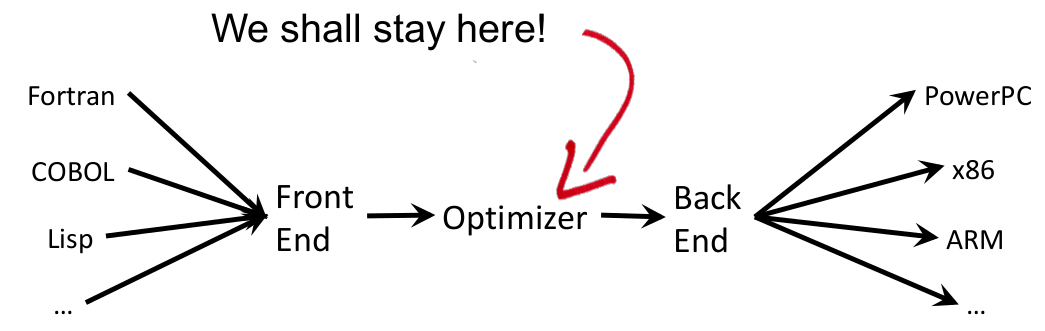
\includegraphics[width=\textwidth]{img/compiler.png}
    \caption{Basic structure of the compiler.}
    \label{fig:compiler}
\end{figure}

\section{Static vs Dynamic Analysis}
\label{sec:analysis}

Static analysis and dynamic analysis are two different approaches used in software testing and analysis. Next, we will discuss the pros and cons of each other.

\textbf{Static analysis} involves examining the source code, design documents, or other artifacts of a software system without executing the code. It focuses on finding defects, vulnerabilities, or potential issues by analyzing the code structure, syntax, and semantics. This analysis is typically performed using specialized tools that can automatically analyze the codebase.

Advantages of Static Analysis:

\begin{itemize}
    \item \textbf{Early bug detection:} Static analysis can identify potential issues in the codebase before the software is even executed, allowing for early bug detection and prevention.
    \item \textbf{Scalability:} It can be applied to large codebases and complex systems, making it suitable for projects of various sizes.
    \item \textbf{Automation:} Static analysis tools can automatically analyze the code, making it efficient for finding common coding mistakes and security vulnerabilities.
    \item \textbf{Code quality improvement:} Static analysis can enforce coding standards and best practices, leading to improved code quality and maintainability.
\end{itemize}

Limitations of Static Analysis:

\begin{itemize}
    \item \textbf{Limited runtime information:} Static analysis cannot capture the complete runtime behavior of the software, making it challenging to detect certain types of issues that only manifest during execution.
    \item \textbf{False positives and negatives:} Static analysis tools may produce false positives (flagging code as problematic when it's not) or false negatives (missing actual issues in the code), requiring manual review and validation.
\end{itemize}

\textbf{Dynamic analysis} involves executing the software and observing its behavior in various scenarios. It aims to uncover defects, performance bottlenecks, memory leaks, and other runtime issues. Dynamic analysis typically requires running the software with specific inputs or test cases to exercise different paths and behaviors.

Advantages of Dynamic Analysis:

\begin{itemize}
    \item \textbf{Real-world simulation:} Dynamic analysis provides insights into how the software behaves in real-world scenarios, helping identify issues that might not be apparent through static analysis alone.
    \item \textbf{Coverage of runtime behaviors:} It captures actual runtime behavior, allowing for the detection of issues related to timing, concurrency, memory management, and interactions with external systems.
    \item \textbf{Profiling and performance analysis:} Dynamic analysis tools can measure performance metrics, such as execution time and memory usage, and help identify performance bottlenecks.
\end{itemize}

Limitations of Dynamic Analysis:

\begin{itemize}
    \item \textbf{Late bug detection:} Dynamic analysis detects issues during or after execution, which means that bugs may go undetected until the software is executed.
    \item \textbf{Incomplete coverage:} It may be challenging to exercise all possible execution paths, making it difficult to achieve complete coverage of the software.
    \item \textbf{Time-consuming:} Dynamic analysis requires executing the software, which can be time-consuming, especially for large systems or complex test scenarios.
\end{itemize}

In practice, both static and dynamic analysis techniques complement each other and are often used in combination to achieve comprehensive software testing and analysis. Static analysis helps catch potential issues early in the development process, while dynamic analysis provides insights into the actual runtime behavior and helps uncover issues that may only manifest during execution. 

In this book, we will focus on techniques for static analysis, but there will be a release in the future, a book where It focuses on dynamic analysis. 

\subsection{Program Optimization}

Program optimization refers to the process of improving the performance, efficiency, or other desired characteristics of a software program. Optimization techniques aim to reduce the program's resource usage, such as CPU time, memory consumption, or network bandwidth, while still achieving the desired functionality. Here's an example to illustrate program optimization:

Let's consider a simple example of a function that calculates the sum of numbers in an array using a basic iterative approach:

\begin{lstlisting}[language=Python]
def sum_array(arr):
    result = 0
    for num in arr:
        result += num
    return result
\end{lstlisting}

While this code works correctly, it may not be optimal in terms of performance. If the array has a large number of elements, the iterative approach can be inefficient. We can optimize this code by using a more efficient algorithm, such as a divide-and-conquer approach. Here's an optimized version using recursion:

\begin{lstlisting}[language=Python]
def sum_array_optimized(arr):
    if len(arr) == 1:
        return arr[0]
    else:
        mid = len(arr) // 2
        left_sum = sum_array_optimized(arr[:mid])
        right_sum = sum_array_optimized(arr[mid:])
        return left_sum + right_sum
\end{lstlisting}

In this optimized code, we divide the array into smaller halves recursively until we reach arrays of size 1. Then, we sum the elements of each small array and return the final result. This approach reduces the number of operations required and can be more efficient for large arrays.

It's important to note that program optimization may involve trade-offs. While optimization can improve certain aspects of the program, it may also make the code more complex or harder to understand. This is one of the goals of the techniques that we will see in this book is to optimize programs without the programmer interfering in the code. 

There are many ways to optimize programs. We will see some of these techniques:

\begin{itemize}
    \item Copy elimination
    \item Constant propagation
    \item Lazy Code Motion
    \item Register Allocation
    \item Loop Unrolling
    \item Value Numbering
    \item Strength Reduction
    \item and others more
\end{itemize}

\subsection{Bug Finding}
\label{subsec:bug}

Bug finding refers to the process of identifying and fixing bugs, defects, or errors in software applications. Bugs can cause the software to behave unexpectedly, produce incorrect results, or crash. Bug finding techniques are used to locate and diagnose these issues, allowing developers to resolve them and improve the overall quality and reliability of the software. 

Static analysis tools analyzes the source code or other artifacts without executing the software. They perform automated checks for coding errors, potential bugs, or violations of coding standards. These tools can identify issues such as uninitialized variables, dead code, buffer overflows, or potential security vulnerabilities. Static analysis can be an effective way to catch bugs early in the development process. By the other hand, Dynamic analysis techniques involve running the software with specific inputs or test cases to observe its behavior during execution. These techniques include techniques like runtime monitoring, profiling, and memory analysis. Dynamic analysis can uncover bugs related to performance bottlenecks, memory leaks, concurrency issues, or unexpected behavior during runtime.

Therefore, Compiler analyses are very useful to fine, and sometimes fix, bugs in programs. For example, The snippet code in C++ below there is a security bug. Could you spot a security bug in this program? Don't worry if you could not, the answer it'll be shown during the book.

\begin{lstlisting}[language=C++]
void read_matrix(int* data, char w, char h) {
    char burf_size = w * h;
    if (buf_size < BUF_SIZE) {
        int c0, c1;
        int buf[BUF_SIZE];
        for (c0 = 0; c0 < h; c0++) {
            for (c1 = 0; c1 < w; c1++) {
                int index = c0 * w + c1;
                buf[index] = data[index];
            }
        }
        process(buf);
    }
}
\end{lstlisting}

The main topics when you study static program analyses about the bug finding, but not limited, are:

\begin{itemize}
    \item Null pointer deference
    \item Array out-of-bounds access
    \item Invalid Class Cast
    \item Tainted Flow Vulnerabilities
    \item Integer Overflows
    \item Information leaks
\end{itemize}

\subsection{Introduction to LLVM}
\label{subsec:intro_llvm}

LLVM (Low-Level Virtual Machine) is an open-source compiler infrastructure project that provides a collection of modular compiler and toolchain technologies. Originally developed at the University of Illinois at Urbana-Champaign by Chris Lattner, LLVM has grown into a widely adopted framework for building compilers, code optimization tools, and runtime environments. 

The Key Components of LLVM are:

\begin{itemize}
    \item \textbf{LLVM Core:} The core component of LLVM is a collection of libraries and APIs that provide the foundation for building compilers and other tools. It includes components for front-end parsing, intermediate representation (IR) generation, optimization, and code generation.
    \item \textbf{Clang:} Clang is a front-end C, C++, and Objective-C compiler built using LLVM. It aims to provide high-quality diagnostics, fast compilation, and compatibility with various C/C++ standards. Clang leverages LLVM's modular architecture and infrastructure, making it a popular choice for many developers.
    \item \textbf{LLVM IR:} LLVM uses an intermediate representation (IR) called LLVM IR. It is a platform-independent, typed, and low-level representation of code that sits between the source code and the machine code. LLVM IR allows for various optimizations to be performed on the code before generating the final machine code.
    \item \textbf{Optimization Framework:} LLVM provides a powerful optimization framework that performs a wide range of program transformations to improve code quality and performance. It includes optimizations such as constant propagation, loop optimizations, inlining, dead code elimination, and many others.
    \item \textbf{Just-in-Time Compilation (JIT):} LLVM supports Just-in-Time Compilation, allowing dynamic compilation and execution of code at runtime. This is particularly useful in dynamic languages and environments where code needs to be compiled and optimized on the fly.
    \item \textbf{Target Backends:} LLVM supports multiple target architectures and provides backends for generating machine code for different hardware platforms. This allows LLVM to be used for compiling code for various processors, including x86, ARM, MIPS, PowerPC, and more.
    \item \textbf{Toolchain Integration:} LLVM integrates with various development tools and platforms, making it possible to use LLVM as part of a complete toolchain. It can be integrated with build systems, debuggers, profilers, and other development tools.
\end{itemize}

LLVM is widely used in both academia and industry for various purposes, including compiler research, language implementation, code optimization, and tool development. Its modular and flexible architecture, along with its extensive optimization capabilities, make it a popular choice for building high-performance compilers and software tools. Let's see how to install in your machine in the next section.

\subsection{Installing LLVM}

We suppose that you use an OS based on the Linux kernel. You can use WSL from Windows as well. For user's Apple, the process is pretty similar on Linux.
Your first step is to clone the LLVM from GitHub with the command below:

\begin{verbatim}
    $ git clone https://github.com/llvm/llvm-project
\end{verbatim}

Next step, It'll created inside the llvm-project directory, the build folder. 

\begin{verbatim}
    $ mkdir -p build
\end{verbatim}

After that, we will compile using the CMakefile builder. The command below will build using this build:

\begin{verbatim}
    $ cmake -DLLVM_ENABLE_PROJECTS="clang;clang-tools;
    compiler-rt" -DCMAKE_BUILD_TYPE=Debug -G "Unix Makefiles" ../llvm
\end{verbatim}

Or you can use the Ninja builder:

\begin{verbatim}
    $ cmake -DLLVM_ENABLE_PROJECTS="clang;clang-tools;
    compiler-rt" -DCMAKE_BUILD_TYPE=Debug -G "Ninja" ../llvm
\end{verbatim}

This process takes a long time. With a good machine, several cores, and a lot of RAM memory, this process can take approximately 20–30 minutes. After this process, congratulation on your machine you have installed LLVM, and you're ready for the next chapter. 

Any doubts about the process, you can read the getting started from \hyperlink{https://llvm.org/docs/GettingStarted.html}{LLVM page}.
\chapter{Control Flow Graph}
\label{ch:cfg}

A Control Flow Graph (CFG) is a graphical representation of the control flow or flow of execution within a program. It illustrates how the program's instructions or statements are connected and executed based on various control structures such as conditionals (if-else statements), loops (for, while statements), and function calls.

In a CFG, each node represents a basic block, which is a sequence of instructions with a single entry point and a single exit point. The nodes are connected by directed edges that represent the flow of control between the basic blocks. The edges indicate the order in which the basic blocks are executed. Figure \ref{fig:cfg_numbers} presents an example of CFG.

\begin{figure}[!ht]
    \centering
    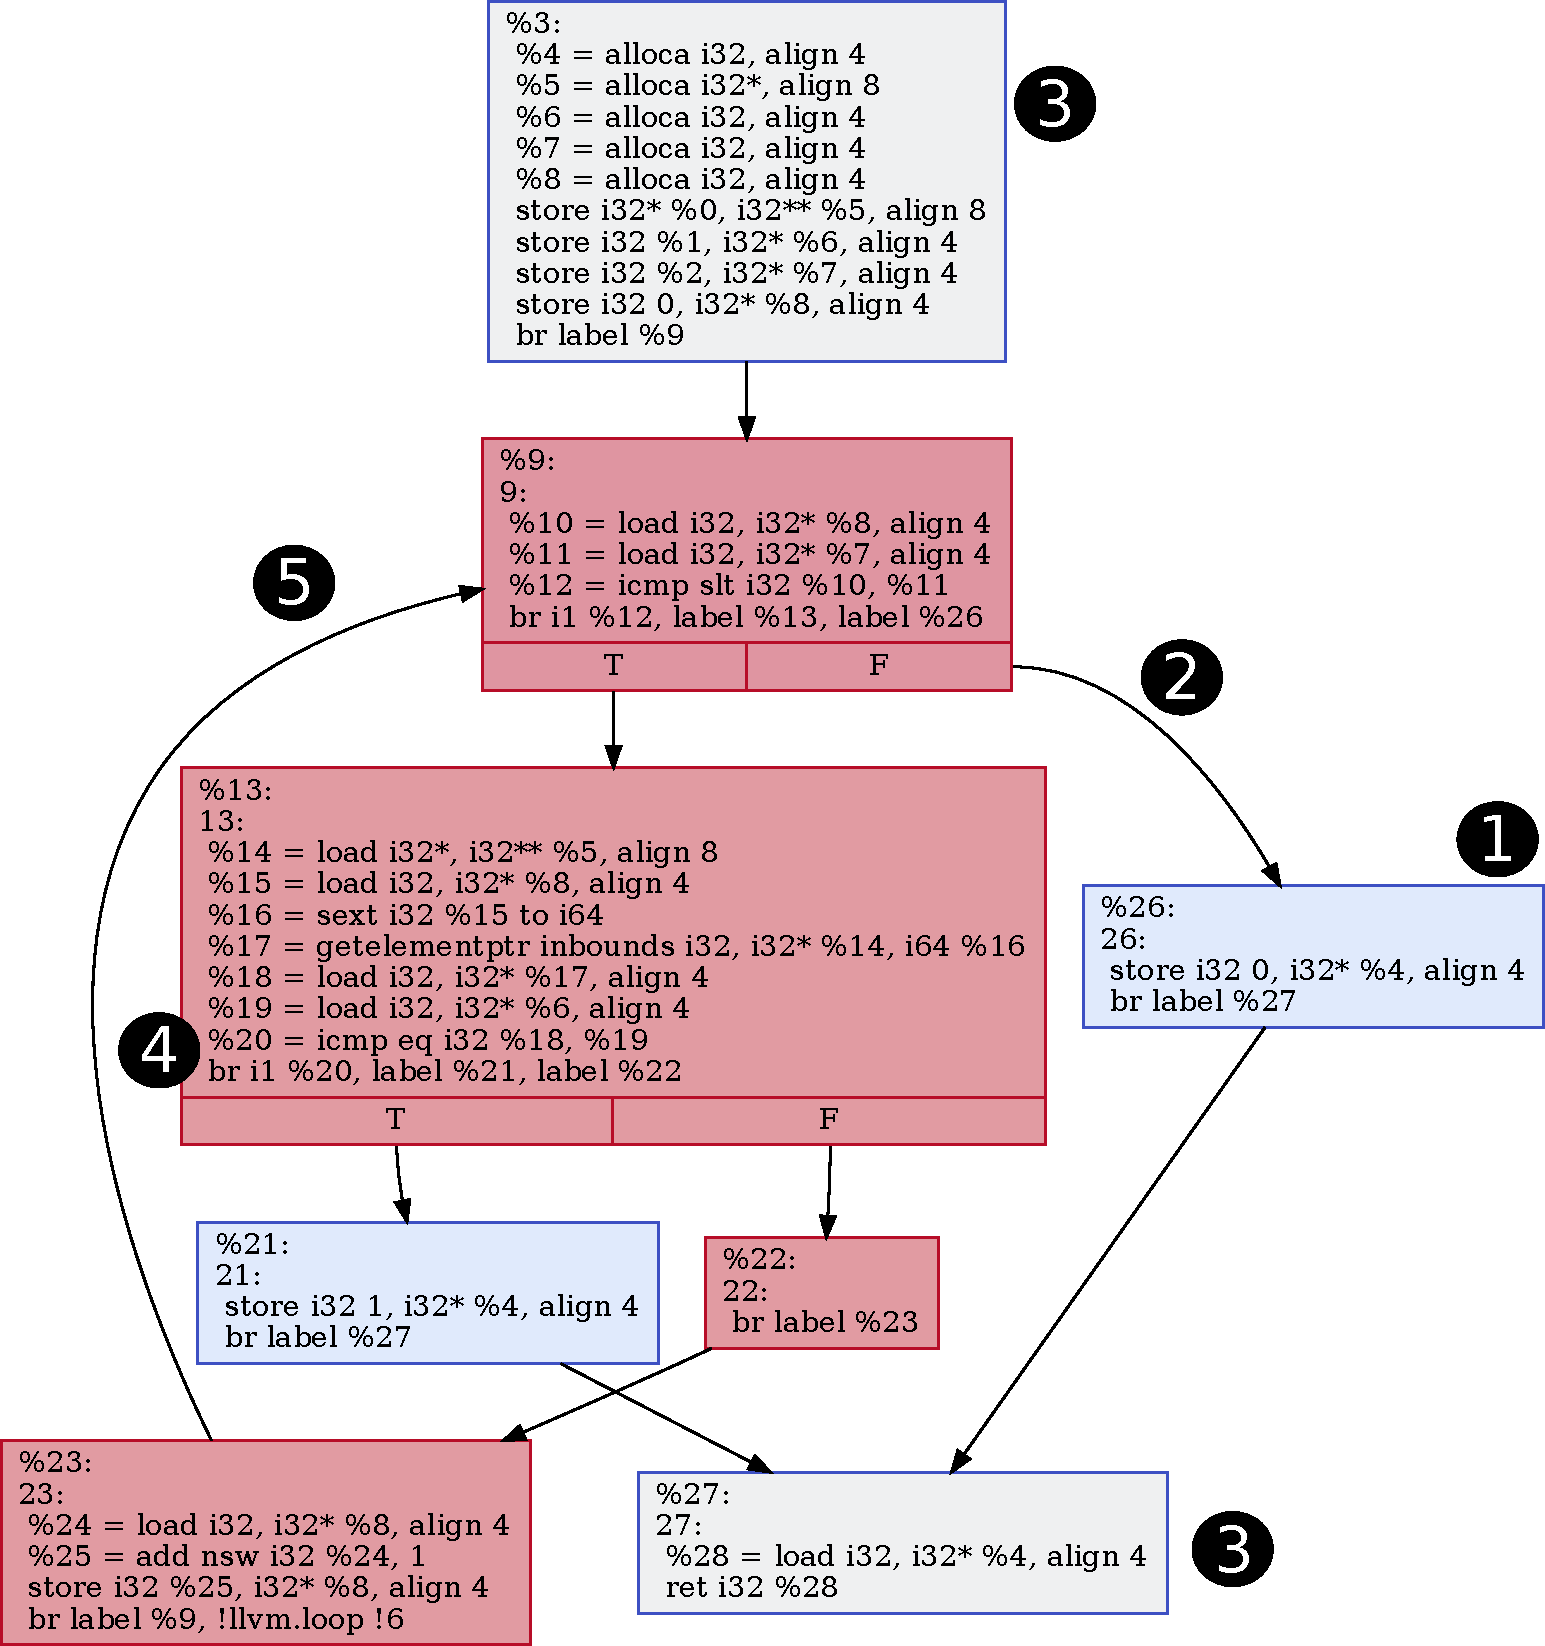
\includegraphics[width=0.95\textwidth]{images/cfg_numbers.pdf}
    \caption{CFG's example}
    \label{fig:cfg_numbers}
\end{figure}

The key components of a Control Flow Graph are: 

\begin{enumerate}
    \item \textbf{Nodes/Basic Blocks:} Each node in the CFG represents a basic block, which is a sequence of instructions with a single entry point and a single exit point. A basic block typically consists of a straight-line sequence of instructions without any branches.
    \item \textbf{Edges:} The edges in the CFG represent the flow of control between the basic blocks. They show how the program transitions from one basic block to another based on the execution of statements such as conditionals, loops, or function calls.
    \item \textbf{Entry and Exit Nodes:} The entry node represents the starting point of the program, and the exit node represents the endpoint or termination of the program. These nodes are connected to the rest of the CFG and provide the overall structure of the control flow.
    \item \textbf{Branching Statements:} Conditional statements, such as if-else or switch statements, introduce branches in the control flow. Branches create multiple paths in the CFG, leading to different basic blocks depending on the evaluated conditions.
    \item \textbf{Loops:} Loop statements, such as for or while loops, introduce repetitive execution in the control flow. The CFG represents loops by creating back edges that connect the exit point of the loop to the entry point, allowing the loop to iterate until the exit condition is met.
\end{enumerate}

CFGs are commonly used in program analysis, optimization, and debugging. They provide a visual representation of the program's control flow, enabling developers and researchers to analyze the program's behavior, identify potential issues, understand code coverage, and perform optimizations or transformations on the program's control flow structure. CFGs are particularly useful for understanding complex programs with multiple control structures and decision points.

\subsection{Generating CFGs with LLVM}

LLVM provides a powerful infrastructure for generating Control Flow Graphs (CFGs) for programs. The LLVM framework, along with its intermediate representation (IR) and associated tools, can be used to analyze and visualize the control flow of code.

The code which we will use as an example will be this:

\begin{lstlisting}[language=C++]
void foo(int** a, int N) {
    int i, j;
    for (i = 0; i < N; i++) {
        for (j = 0; j < N; j++) {
            a[i][j] = 0;
        }
    }
    for (i = 0; i < N; i++) {
        a[i][i] = 1;
    }
}
\end{lstlisting}

First, you need to compile your source code to LLVM IR using the LLVM compiler, such as Clang. Clang can generate LLVM IR from various programming languages like C, C++, and Swift. Use the appropriate compiler flags to emit the LLVM IR instead of generating object files or executables. Example:

\begin{verbatim}
    $ clang -Xclang -disable-O0-optnone -S -emit-llvm foo.c -o foo.ll
\end{verbatim}

Once you have the LLVM IR file, you can use LLVM's API or tools to load and manipulate the IR. The LLVM C++ API provides rich functionality for working with IR, and various command-line tools like \textbf{llvm-dis}, \textbf{llvm-as}, or \textbf{opt} can be used to process the IR. We will use the opt command:

\begin{verbatim}
    $ opt -dot-cfg foo.ll -disable-output
\end{verbatim}

Once you have built the CFG, you can either visualize it graphically or perform further analysis or transformations. There are various graph visualization tools available, such as Graphviz or the LLVM dot tool, which can generate graphical representations of the CFG.

Example command to generate a graphical CFG using LLVM's dot tool:

\begin{verbatim}
    $ dot -Tpdf .foo.dot -o foo.pdf
\end{verbatim}

In the end, the result is shown in Figure \ref{fig:cfg_foo}. Remember to refer to the LLVM documentation, tutorials, and examples for more detailed information on using the LLVM APIs and tools to generate and work with CFGs.

\begin{figure}[!ht]
    \centering
    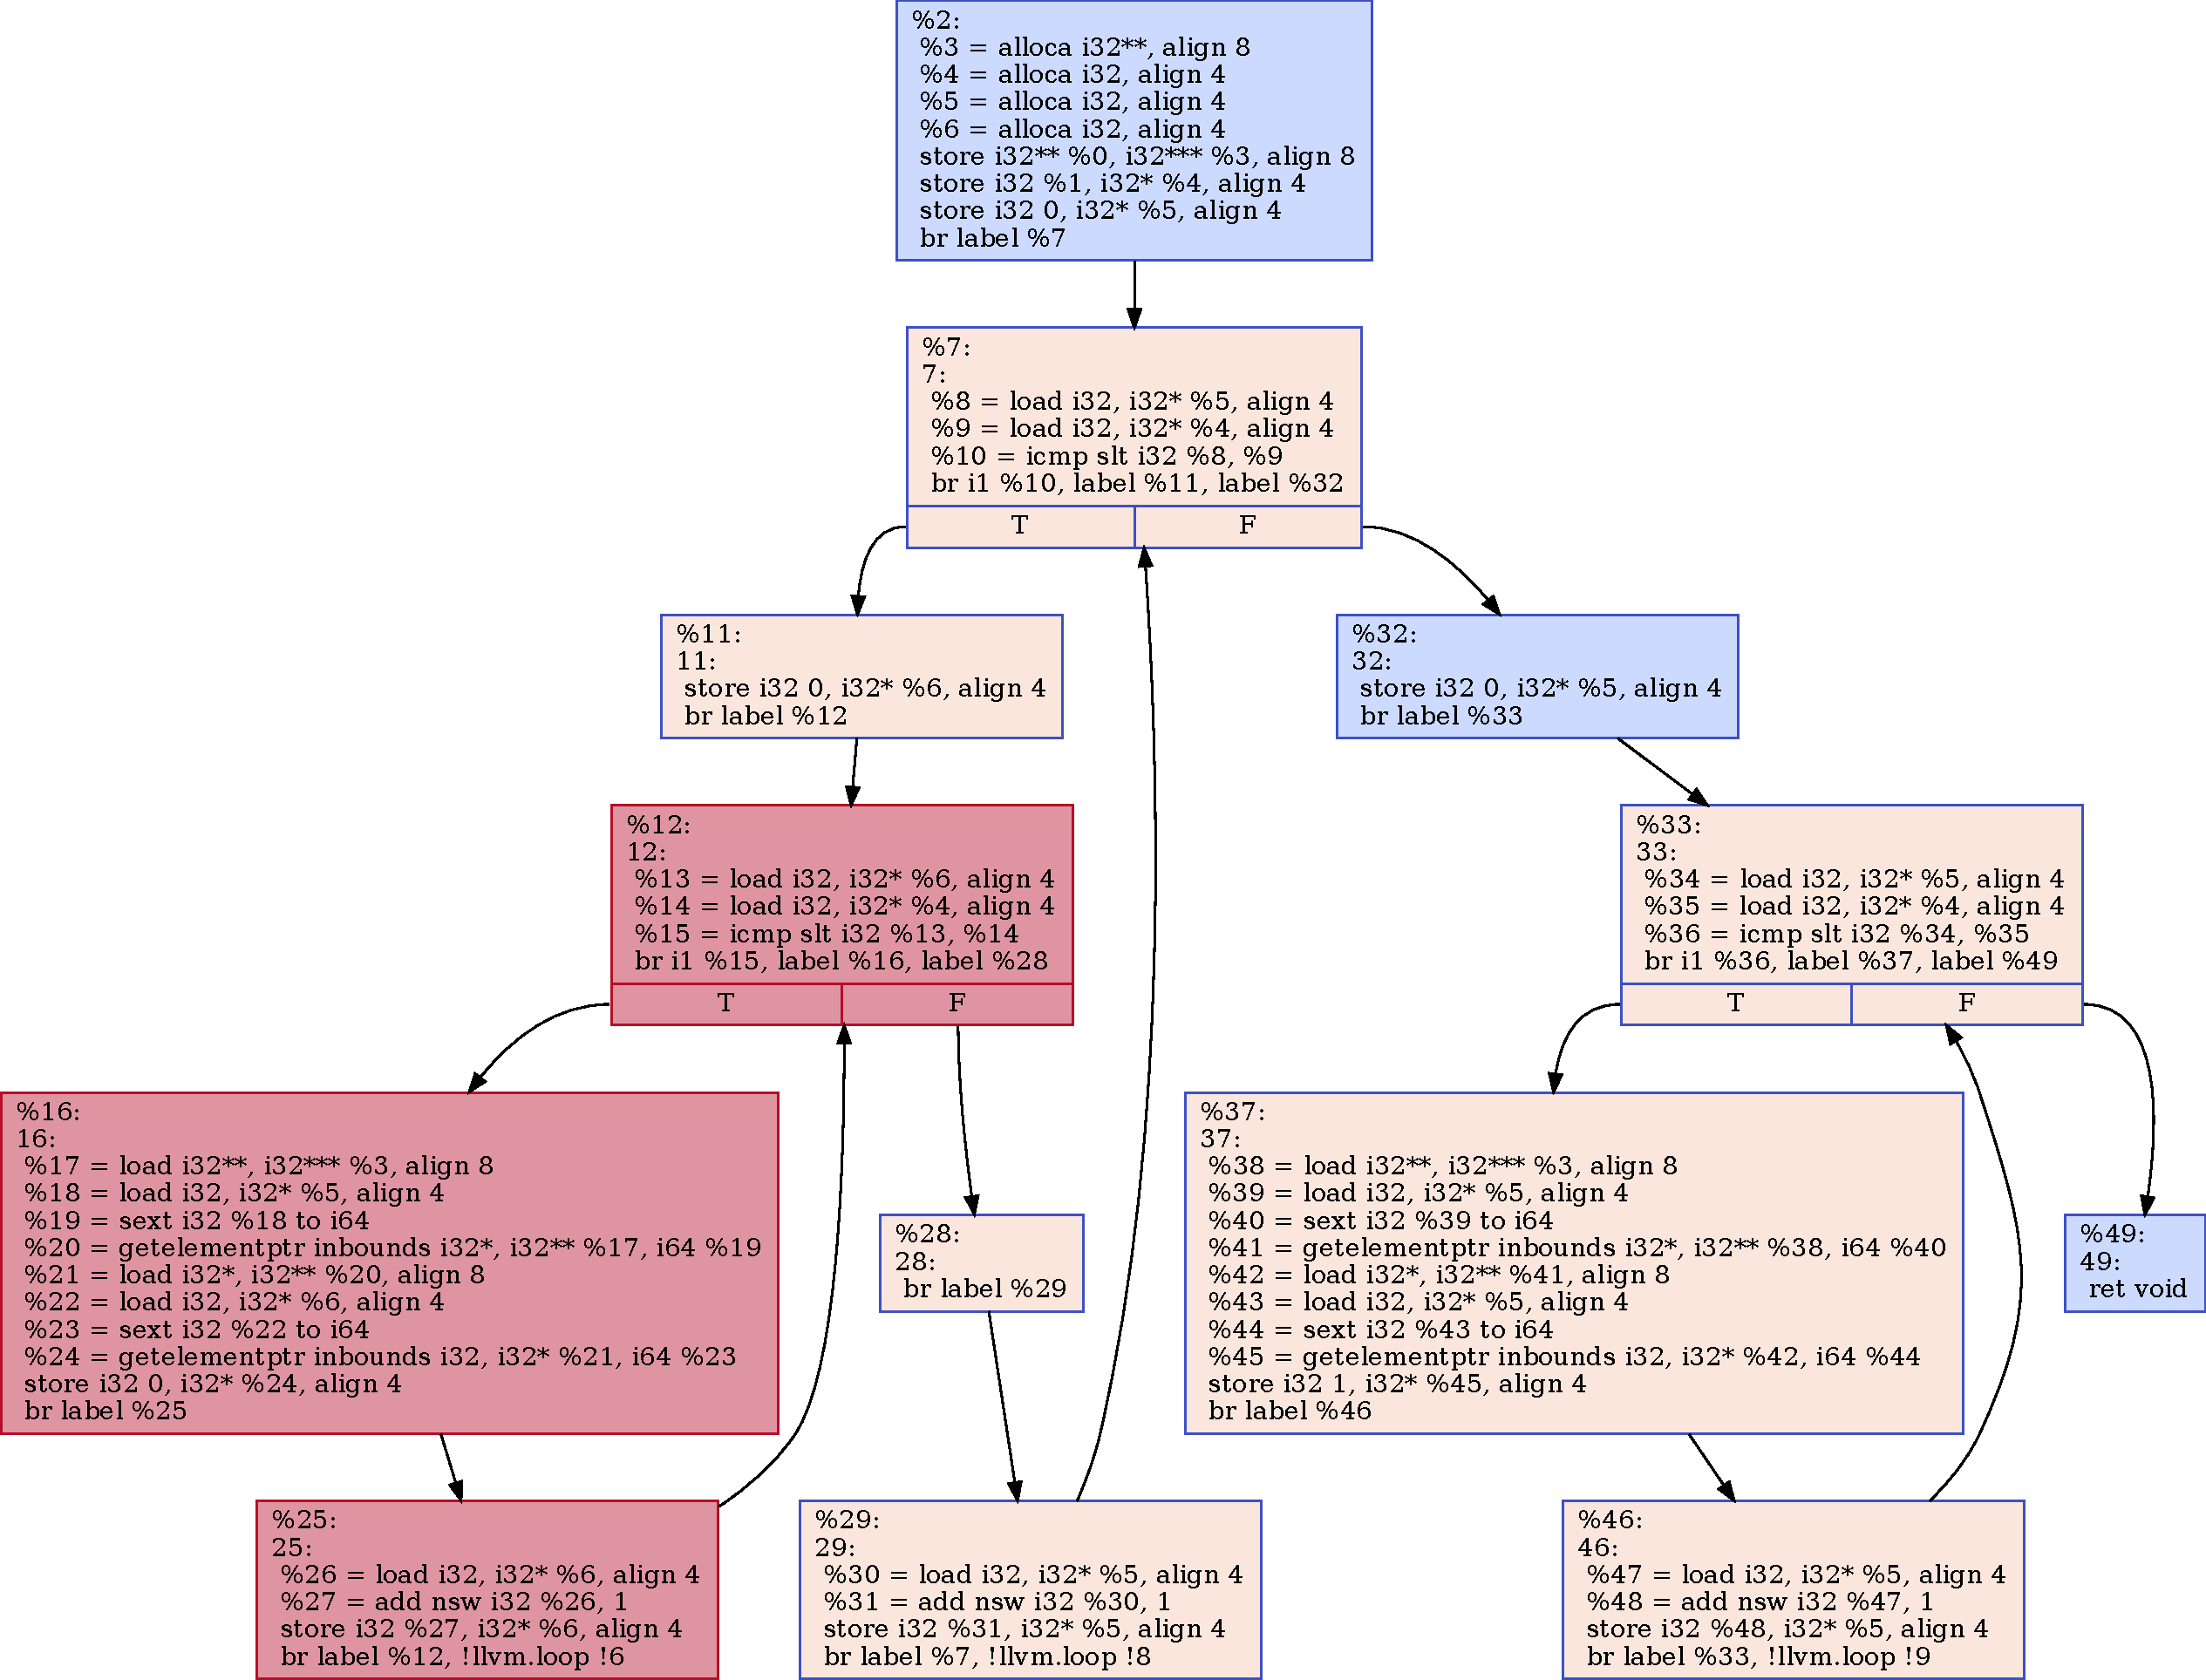
\includegraphics[width=\textwidth]{images/cfg.pdf}
    \caption{CFG's example}
    \label{fig:cfg_foo}
\end{figure}
\chapter{Range Analysis}
\label{ch:range}

Range analysis is a program analysis technique used to determine the possible ranges of values that program variables can take on at different points in a program's execution. The analysis can be performed on different types of variables, such as integers, floating-point numbers, or pointers. Thus, It works by analyzing the operations that are performed on a variable throughout the program's execution. By analyzing the arithmetic and logical operations performed on a variable, range analysis can determine the possible minimum and maximum values that the variable can take on.

For example, consider the following code snippet:

\begin{lstlisting}[language=C++]
int x = 0;
for (int i = 0; i < 100; i++) {
    x += i;
}
\end{lstlisting}

In this code, the variable \textbf{x} is initialized to 0 and is then incremented by the value of \textbf{i} in each iteration of the loop. By analyzing the loop, range analysis can determine that the minimum value of \textbf{x} is 0, when \textbf{i} is 0, and the maximum value of \textbf{x} is 4950, when \textbf{i} is 99.

Range analysis can be used for various program optimizations, such as loop unrolling, array bounds checking elimination, and constant propagation. By providing information about the possible ranges of variable values, range analysis can help optimize programs and improve their performance. However, It is important to note that range analysis is not always precise, and the computed ranges are often conservative (i.e., they may be wider than the actual range of values).

\section{Dead Code Elimination}
\label{sec:dce}

Dead code elimination is a program optimization technique that involves removing code that is never executed during the program's execution. Dead code can be a result of various factors such as redundant code, code that has been commented out, or unreachable code. It can improve the performance of a program by reducing the size of the code that needs to be executed. By removing code that is never executed, the compiler can reduce the amount of memory and CPU time required to execute the program.

The process of dead code elimination involves analyzing the control flow graph of the program to identify code that is never executed. The analysis can be performed statically (i.e., at compile time) or dynamically (i.e., at runtime). Static analysis is more common and involves analyzing the program's source code or intermediate representation (IR) to identify dead code. Dynamic analysis, on the other hand, involves executing the program with input data to identify code that is never executed.

Dead code elimination can also be performed selectively, where only specific parts of the program are analyzed for dead code. For example, in a large program, it may be more practical to analyze a specific module or function for dead code instead of analyzing the entire program.

In addition to improving performance, dead code elimination can also help improve code maintainability by removing unnecessary code that can clutter the program and make it harder to understand. However, care must be taken when applying dead code elimination to avoid removing code that may be used in future development or debugging.

Let's see an example C++ code where dead code elimination can occur:

\begin{lstlisting}[language=C++]
int foo() {
    int x = 10;
    int y = 20;
    int z = 0;

    // This code will never be executed
    if (x == y) {
        z = 30;
    }
    
    return x + y;
}
\end{lstlisting}

In this code, the if statement checks whether x is equal to y and sets z to 30 if they are equal. However, since x is initialized to 10 and y is initialized to 20, the condition of the if statement will never be true, and the code inside the if statement will never be executed.

As a result, the code inside the if statement can be considered dead code, and can be eliminated by the compiler. After dead code elimination, the optimized code would look like this:

\begin{lstlisting}[language=C++]
int foo() {
    int x = 10;
    int y = 20;
    
    return x + y;
}
\end{lstlisting}

In this optimized code, the if statement and the assignment to z have been removed, as they are never executed. This reduces the size of the code and can improve the program's performance.

\section{Array Bounds Check Elimination}
\label{sec:array}

Array bounds check elimination is a program optimization technique that involves removing redundant bounds checking operations on array accesses in a program. Bounds checking is a runtime operation that ensures that array accesses are within the bounds of the array. If array access is out of bounds, it can lead to memory corruption, crashes, or security vulnerabilities. It can improve the performance of a program by reducing the number of bounds checks performed during program execution. This can be particularly useful in performance-critical programs, such as scientific simulations or video games, where small performance improvements can have a significant impact on overall program performance.

The process of array bounds check elimination involves analyzing the program to identify cases where the bounds of array access are known at compile time. For example, if an array access is inside a loop with a constant index value, the bounds of the array access can be determined at compile time. In such cases, the bounds check can be eliminated, and the array access can be performed directly.

Let's see an example C++ code where array bounds check elimination can occur:

\begin{lstlisting}[language=C++]
int foo() {
    const int array_size = 10;
    int array[array_size];
    int choose = 5;

    // Initialize array with values from 0 to 9
    for (int i = 0; i < array_size; i++) {
        array[i] = i;
    }

    // Access array with a constant index value
    if (choose < array_size)
        return array[choose];
    else 
        throw new ArrayIndexOutOfBoundsException()
}
\end{lstlisting}

In this code, the array is initialized with values from 0 to 9, and then the value at index 5 is printed to the console. Since the index value of 5 is known at compile time, the bounds of the array access are also known, and the bounds check can be eliminated. This can result in faster execution of the program, as the program does not have to perform a bounds check on the array access. The optimized code will be transformed as: 

\begin{lstlisting}[language=C++]
int foo() {
    const int array_size = 10;
    int array[array_size];
    int choose = 5;

    // Initialize array with values from 0 to 9
    for (int i = 0; i < array_size; i++) {
        array[i] = i;
    }

    // Access array with a constant index value
    return array[choose];
}
\end{lstlisting}

Array bounds check elimination can be performed automatically by modern compilers, such as GCC and Clang, or manually by the programmer using techniques such as loop unrolling, constant propagation, and array access rewriting.

\section{Integer Overflow Check Elimination}
\label{sec:integerOverflow}


\section{Malign	Integer	Overflows}
\label{sec:malignInteger}


\end{document}
